
% 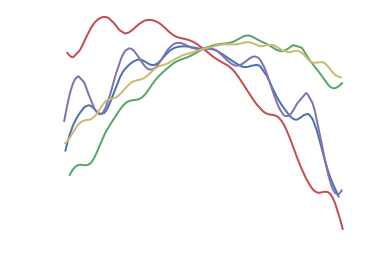
\includegraphics[width=.153\textwidth]{figs/gpSamples/main.png}
\begin{tikzpicture}
% level 2
\node[draw,rectangle, ,minimum width = \textwidth, minimum height = 4cm] (frame) {};
\node[text width = 11.5cm,xshift=-1.1 cm] (mcmc) {$\;\;\;\; \;\;\;\; \;\;P(\mathbf{K})\approx \frac{1}{N}
\sum\limits_{n=1}^N f(\mathbf{K}_n)\;\;\text{where}\, f(\mathbf{K}_n) = \begin{cases}
  1, & \text{if } \mathbf{K} \underset{global}{\in} \mathbf{K}_n, \\
  0, & \text{otherwise}.
\end{cases}$ \vspace{3 mm}

$P(\mathbf{K}_a \land \mathbf{K}_b) \approx\frac{1}{N}
\sum\limits_{n=1}^N f(\mathbf{K}_n)\;\;\text{where}\,f(\mathbf{K}_n) = \begin{cases}
  1, & \text{if } \mathbf{K}_a\, \text{and}\, \mathbf{K}_a  \underset{global}{\in} \mathbf{K}_n, \\
  0, & \text{otherwise}.
\end{cases}$\vspace{3 mm}

$P(\mathbf{K}_a \lor \mathbf{K}_b) = P(\mathbf{K}_a) + P(\mathbf{K}_b) - P(\mathbf{K}_a \land \mathbf{K}_b)$

};
\node[right =0.cm of mcmc] (barplot) {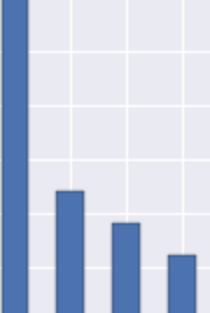
\includegraphics[height=3cm]{figs/barplot.png}};
% level 2
\node[below =1.cm of frame] (hyp) {\normalsize \color{blue} What is the probability of a trend, a recurring pattern {\bf and} noise in the data?};
\node[below = -0.2cm of hyp] (hyp_form) {$P\big((\text{LIN}\lor\text{LIN}\times\text{SE})\land
(\text{PER}\lor\text{PER}\times\text{SE}\lor\text{PER}\times\text{LIN})\land
(\text{WN}\lor\text{LIN}\times\text{WN})\big) = 0.36$};

%level 3
\node[below =.5cm of hyp_form , xshift=-3cm] (trend) {\color{blue} Is there a trend?};
\node[below = -0.2cm of trend] (trend_form) {$P(\text{LIN}\lor\text{LIN}\times\text{SE}) = 0.65$};
\node[below = -0.2cm of trend_form] (trend_png) {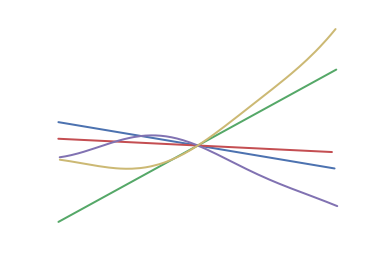
\includegraphics[width=.15\textwidth]{figs/gpSamples/trend.png}};

\node[below =.5cm of hyp_form, xshift=3cm] (noise) {\color{blue} Is there noise? };
\node[below = -0.2cm of noise] (noise_form) {$P(\text{WN}\lor\text{LIN}\times\text{WN}) = 0.75$};
\node[below = -0.2cm of noise_form] (noise_png) {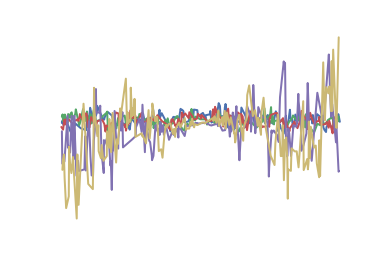
\includegraphics[width=.15\textwidth]{figs/gpSamples/noise.png}};

% level 4
\node[below =.5cm of trend_png , xshift=-2cm] (linear_trend) {\color{blue} A linear trend?};
\node[below = -0.2cm of linear_trend] (linear_trend_form) {$P(\text{LIN}) = 0.63$};
\node[below = -0.2cm of linear_trend_form] (linear_trend_png) {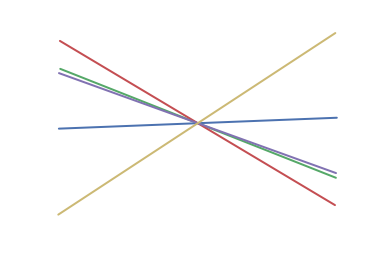
\includegraphics[width=.15\textwidth]{figs/gpSamples/lin.png}};

\node[below =.5cm of trend_png , xshift=1cm] (smooth_trend) {\color{blue} A smooth trend?};
\node[below = -0.2cm of smooth_trend] (smooth_trend_form) {$P(\text{LIN}\times\text{SE}) = 0.02$};
\node[below = -0.2cm of smooth_trend_form] (smooth_trend_png) {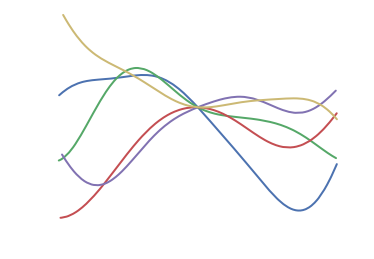
\includegraphics[width=.15\textwidth]{figs/gpSamples/selin.png}};

\node[below =.5cm of noise_png, xshift=-1cm] (het_noise) {\color{blue} Heteroskedastic noise? };
\node[below = -0.2cm of het_noise] (het_noise_form) {$P(\text{LIN}\times\text{WN}) = 0$};
\node[below = -0.2cm of het_noise_form] (het_noise_png) {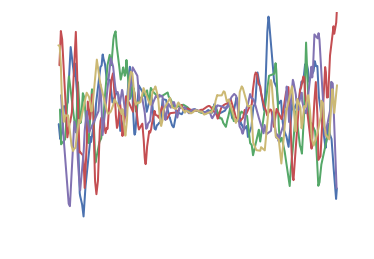
\includegraphics[width=.15\textwidth]{figs/gpSamples/linwn.png}};

\node[below =.5cm of noise_png, xshift=2cm] (white_noise) {\color{blue} White  noise? };
\node[below = -0.2cm of white_noise] (white_noise_form) {$P(\text{WN}) = 0.75$};
\node[below = -0.2cm of white_noise_form] (white_noise_png) {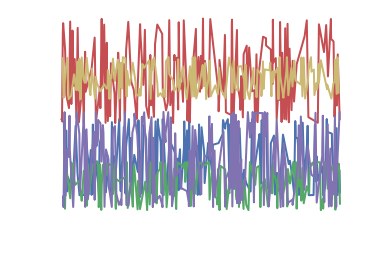
\includegraphics[width=.15\textwidth]{figs/gpSamples/wn.png}};

% level 5
\node[below =6.2cm of hyp_form] (recurring) {\color{blue} Is there repeating structure?};
\node[below = -0.2cm of recurring] (recurring_form) {$P(\text{PER}\lor\text{PER}\times\text{SE}\lor\text{PER}\times\text{LIN}) = 0.73$};
\node[below = -0.2cm of recurring_form] (recurring_png) {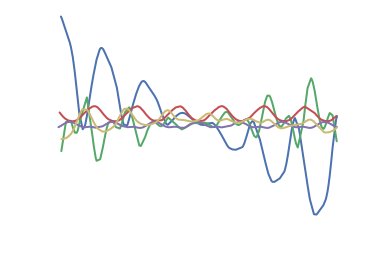
\includegraphics[width=.15\textwidth]{figs/gpSamples/recurring.png}};
%\draw[->,dashed] (barplot) -- (mcmc);

% level 6
\node[below =.5cm of recurring_png] (seper_form) {$\text{PER}\times\text{SE}=0.34$};
\node[below = -0.2cm of seper_form] (seper_png) {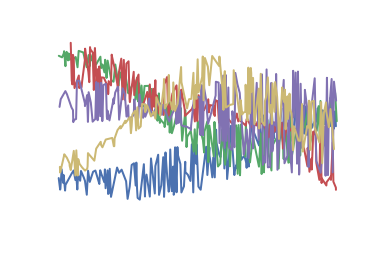
\includegraphics[width=.15\textwidth]{figs/gpSamples/seper.png}};

\node[below =.5cm of recurring_png, xshift=-3cm] (per_form) {$\text{PER}=0.32$};
\node[below = -0.2cm of per_form] (per_png) {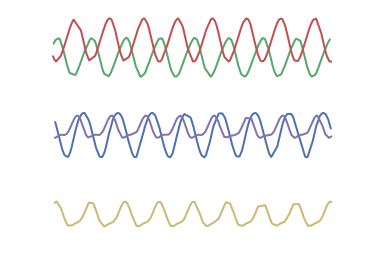
\includegraphics[width=.15\textwidth]{figs/gpSamples/per.png}};

\node[below =.5cm of recurring_png,xshift=3cm] (perlin_form) {$\text{PER}\times\text{LIN}=0.07$};
\node[below = -0.2cm of perlin_form] (seper_png) {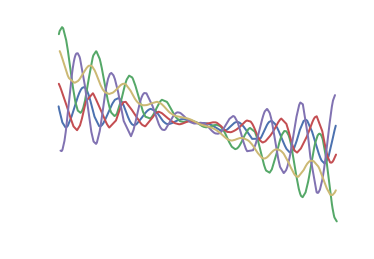
\includegraphics[width=.15\textwidth]{figs/gpSamples/perlin.png}};


\draw[->] (frame) -- (hyp);


\draw[->] (hyp_form) -- (trend);
\draw[->] (hyp_form) -- (noise);
\draw[->] (hyp_form) -- (recurring);


\draw[->] (noise_png) -- (het_noise);
\draw[->] (noise_png) -- (white_noise);

\draw[->] (trend_png) -- (linear_trend);
\draw[->] (trend_png) -- (smooth_trend);

\draw[->] (recurring_png) -- (per_form);
\draw[->] (recurring_png) -- (seper_form);
\draw[->] (recurring_png) -- (perlin_form);


\end{tikzpicture}



%  \multicolumn{3}{c}{$P(\text{PER}\lor\text{PER}\times\text{SE}\lor\text{PER}\times\text{LIN})$}